\section{How I Found the Fandom (Unsigned Long)}

\frame{

\frametitle{\secname}

\begin{columns}
\column{0.5\textwidth}

\begin{wideitemize}
\item<1-> Found furries through con videos
\item<2-> Found some eastern dragons with the word “Long” in their name
\item<3-> Thought about “long” for too long
\item<4-> Realized it’s in my code
\item<5-> Pun was too good---I made a fursona
\end{wideitemize}

\column{0.5\textwidth}
\begin{overprint}
\onslide<1>
\begin{figure}
\centering

\includegraphics[width=\textwidth]{slides/unsigned_long/silvergatomon.png}
\end{figure}
\onslide<2>
\begin{figure}
\centering
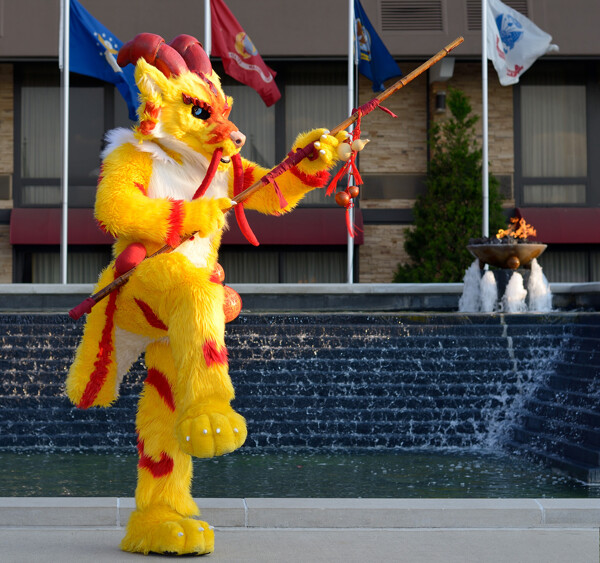
\includegraphics[width=0.8\textwidth]{slides/unsigned_long/tien_long.jpg}

Tien Long
\end{figure}
\onslide<3>
\begin{figure}
\begin{center}
{\fontsize{48}{48}\selectfont l\'ong}\\
{\fontsize{96}{96}\selectfont
\begin{CJK*}{UTF8}{gbsn}
龙
\end{CJK*}
}
\end{center}
\end{figure}
\onslide<4>
\begin{figure}
\centering
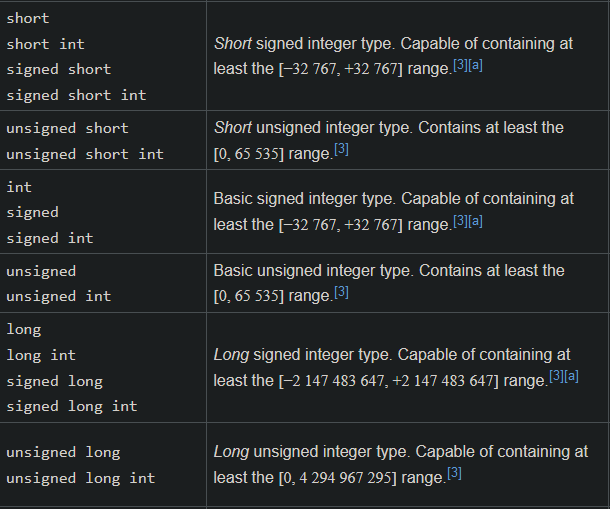
\includegraphics[width=0.9\textwidth]{slides/unsigned_long/data_types.png}
\end{figure}

\onslide<5>

\begin{figure}
\centering
% \vspace{2\baselineskip}
% 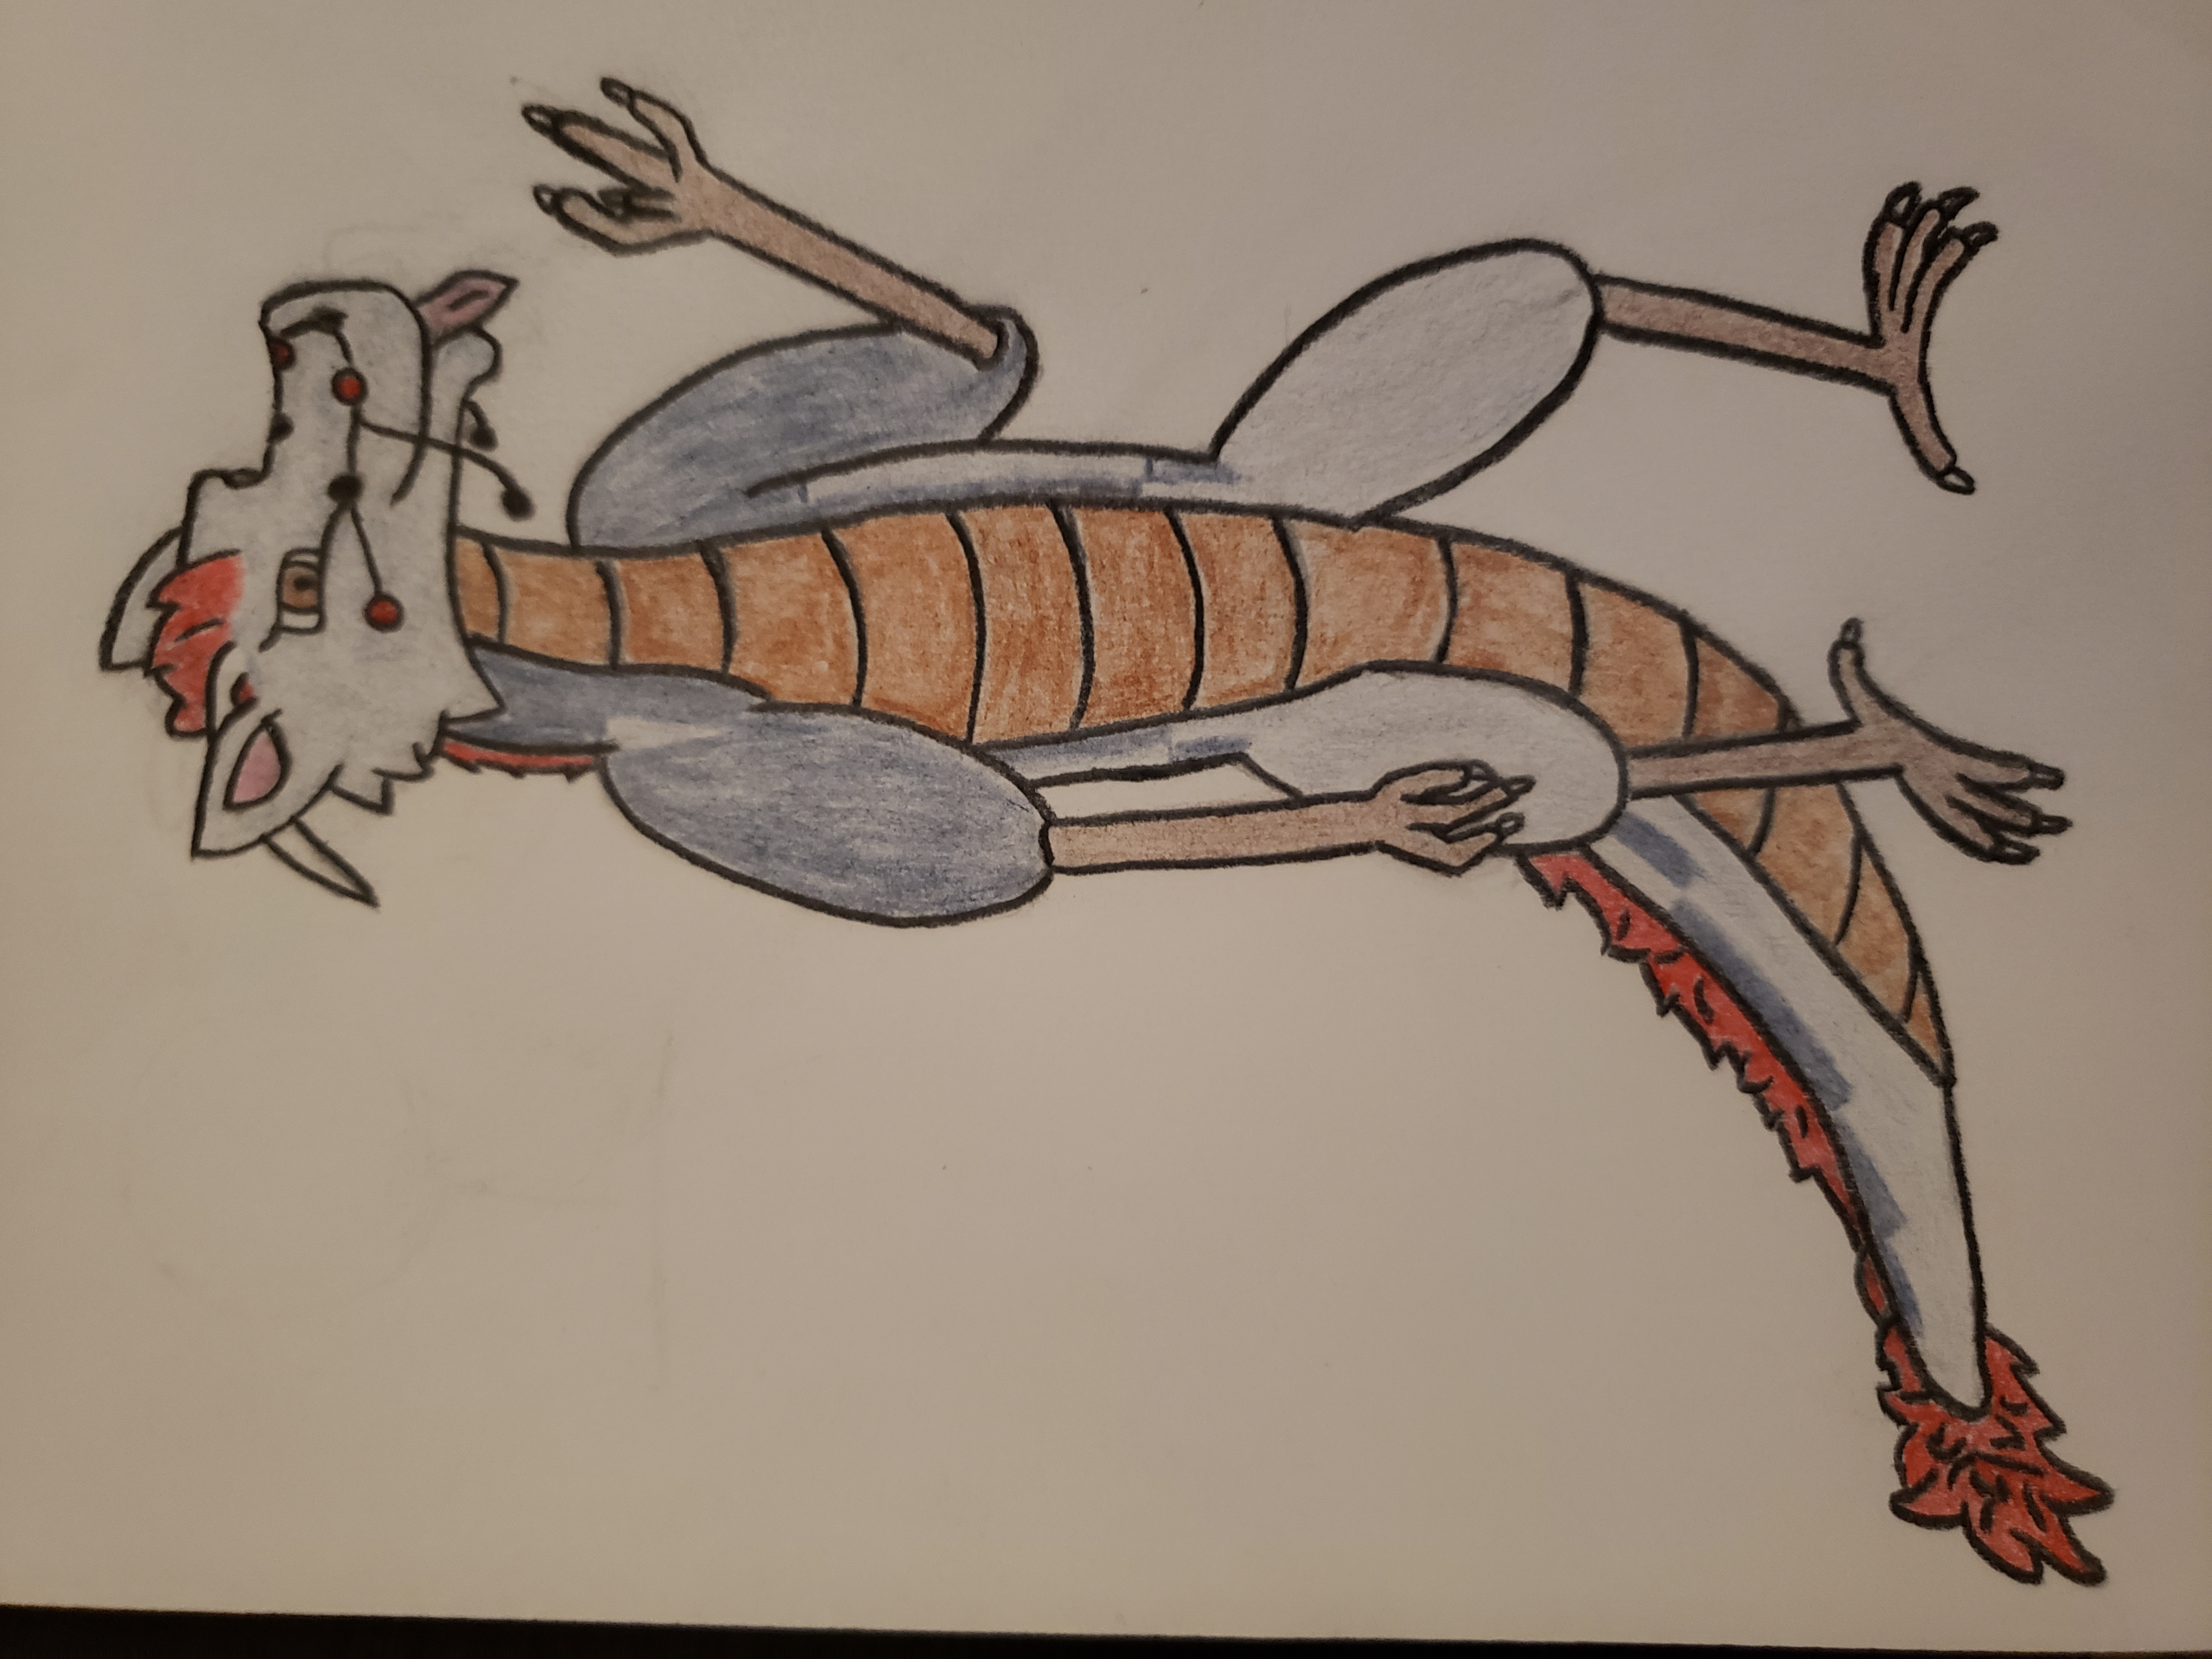
\includegraphics[width=0.57\textwidth,angle=270,origin=rb]{slides/unsigned_long/refsheet_front.jpg}
% \scalebox{-1}[1]{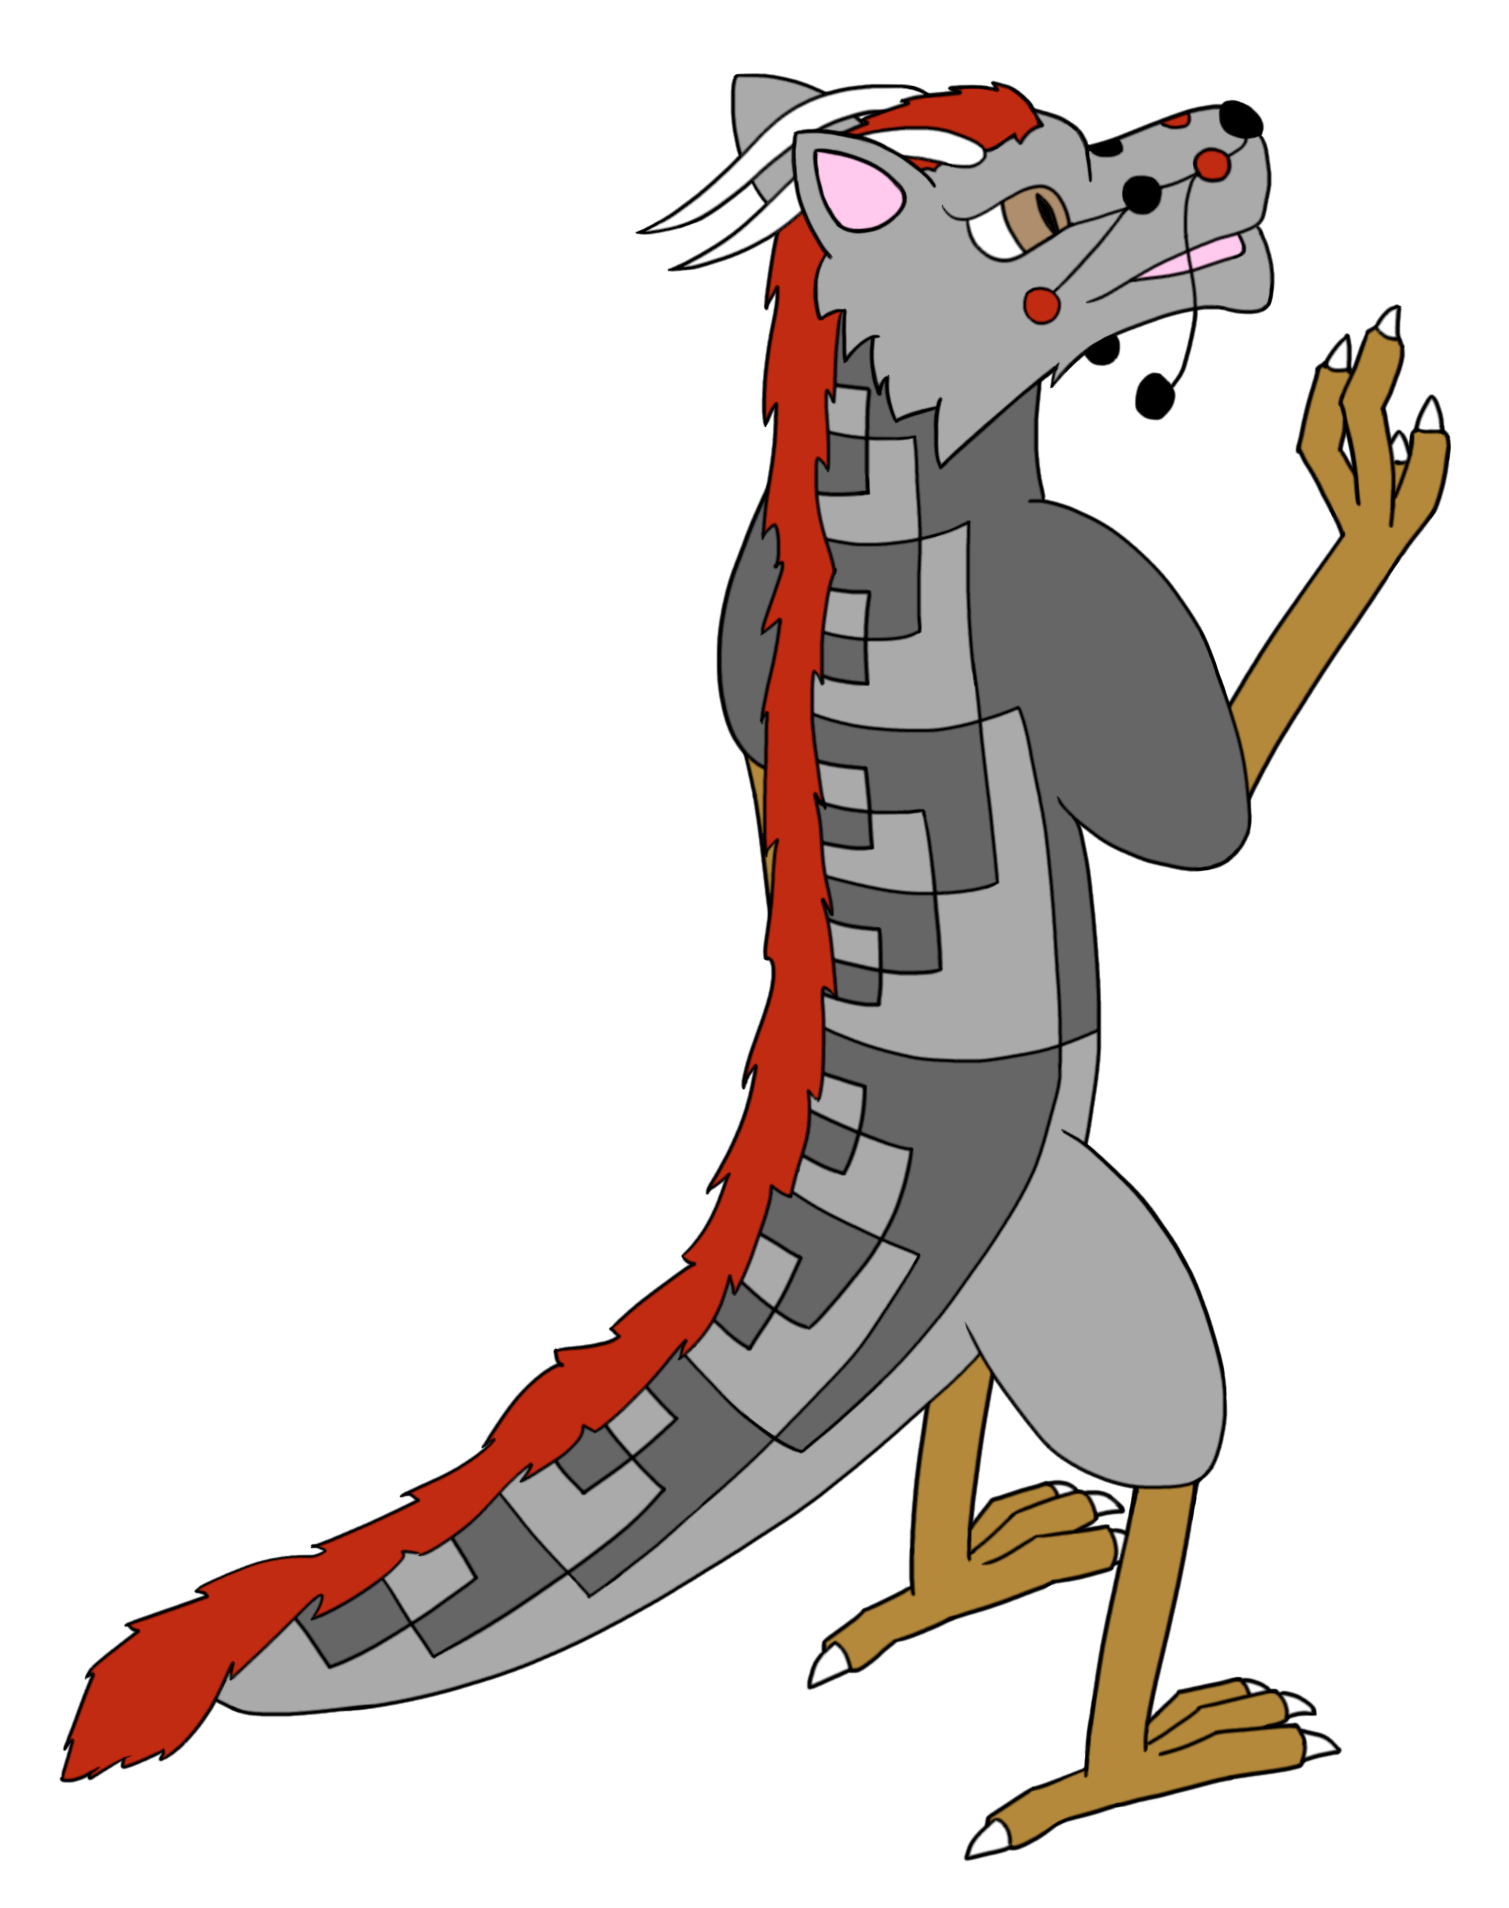
\includegraphics[width=0.43\textwidth]{slides/unsigned_long/refsheet_back.png}}
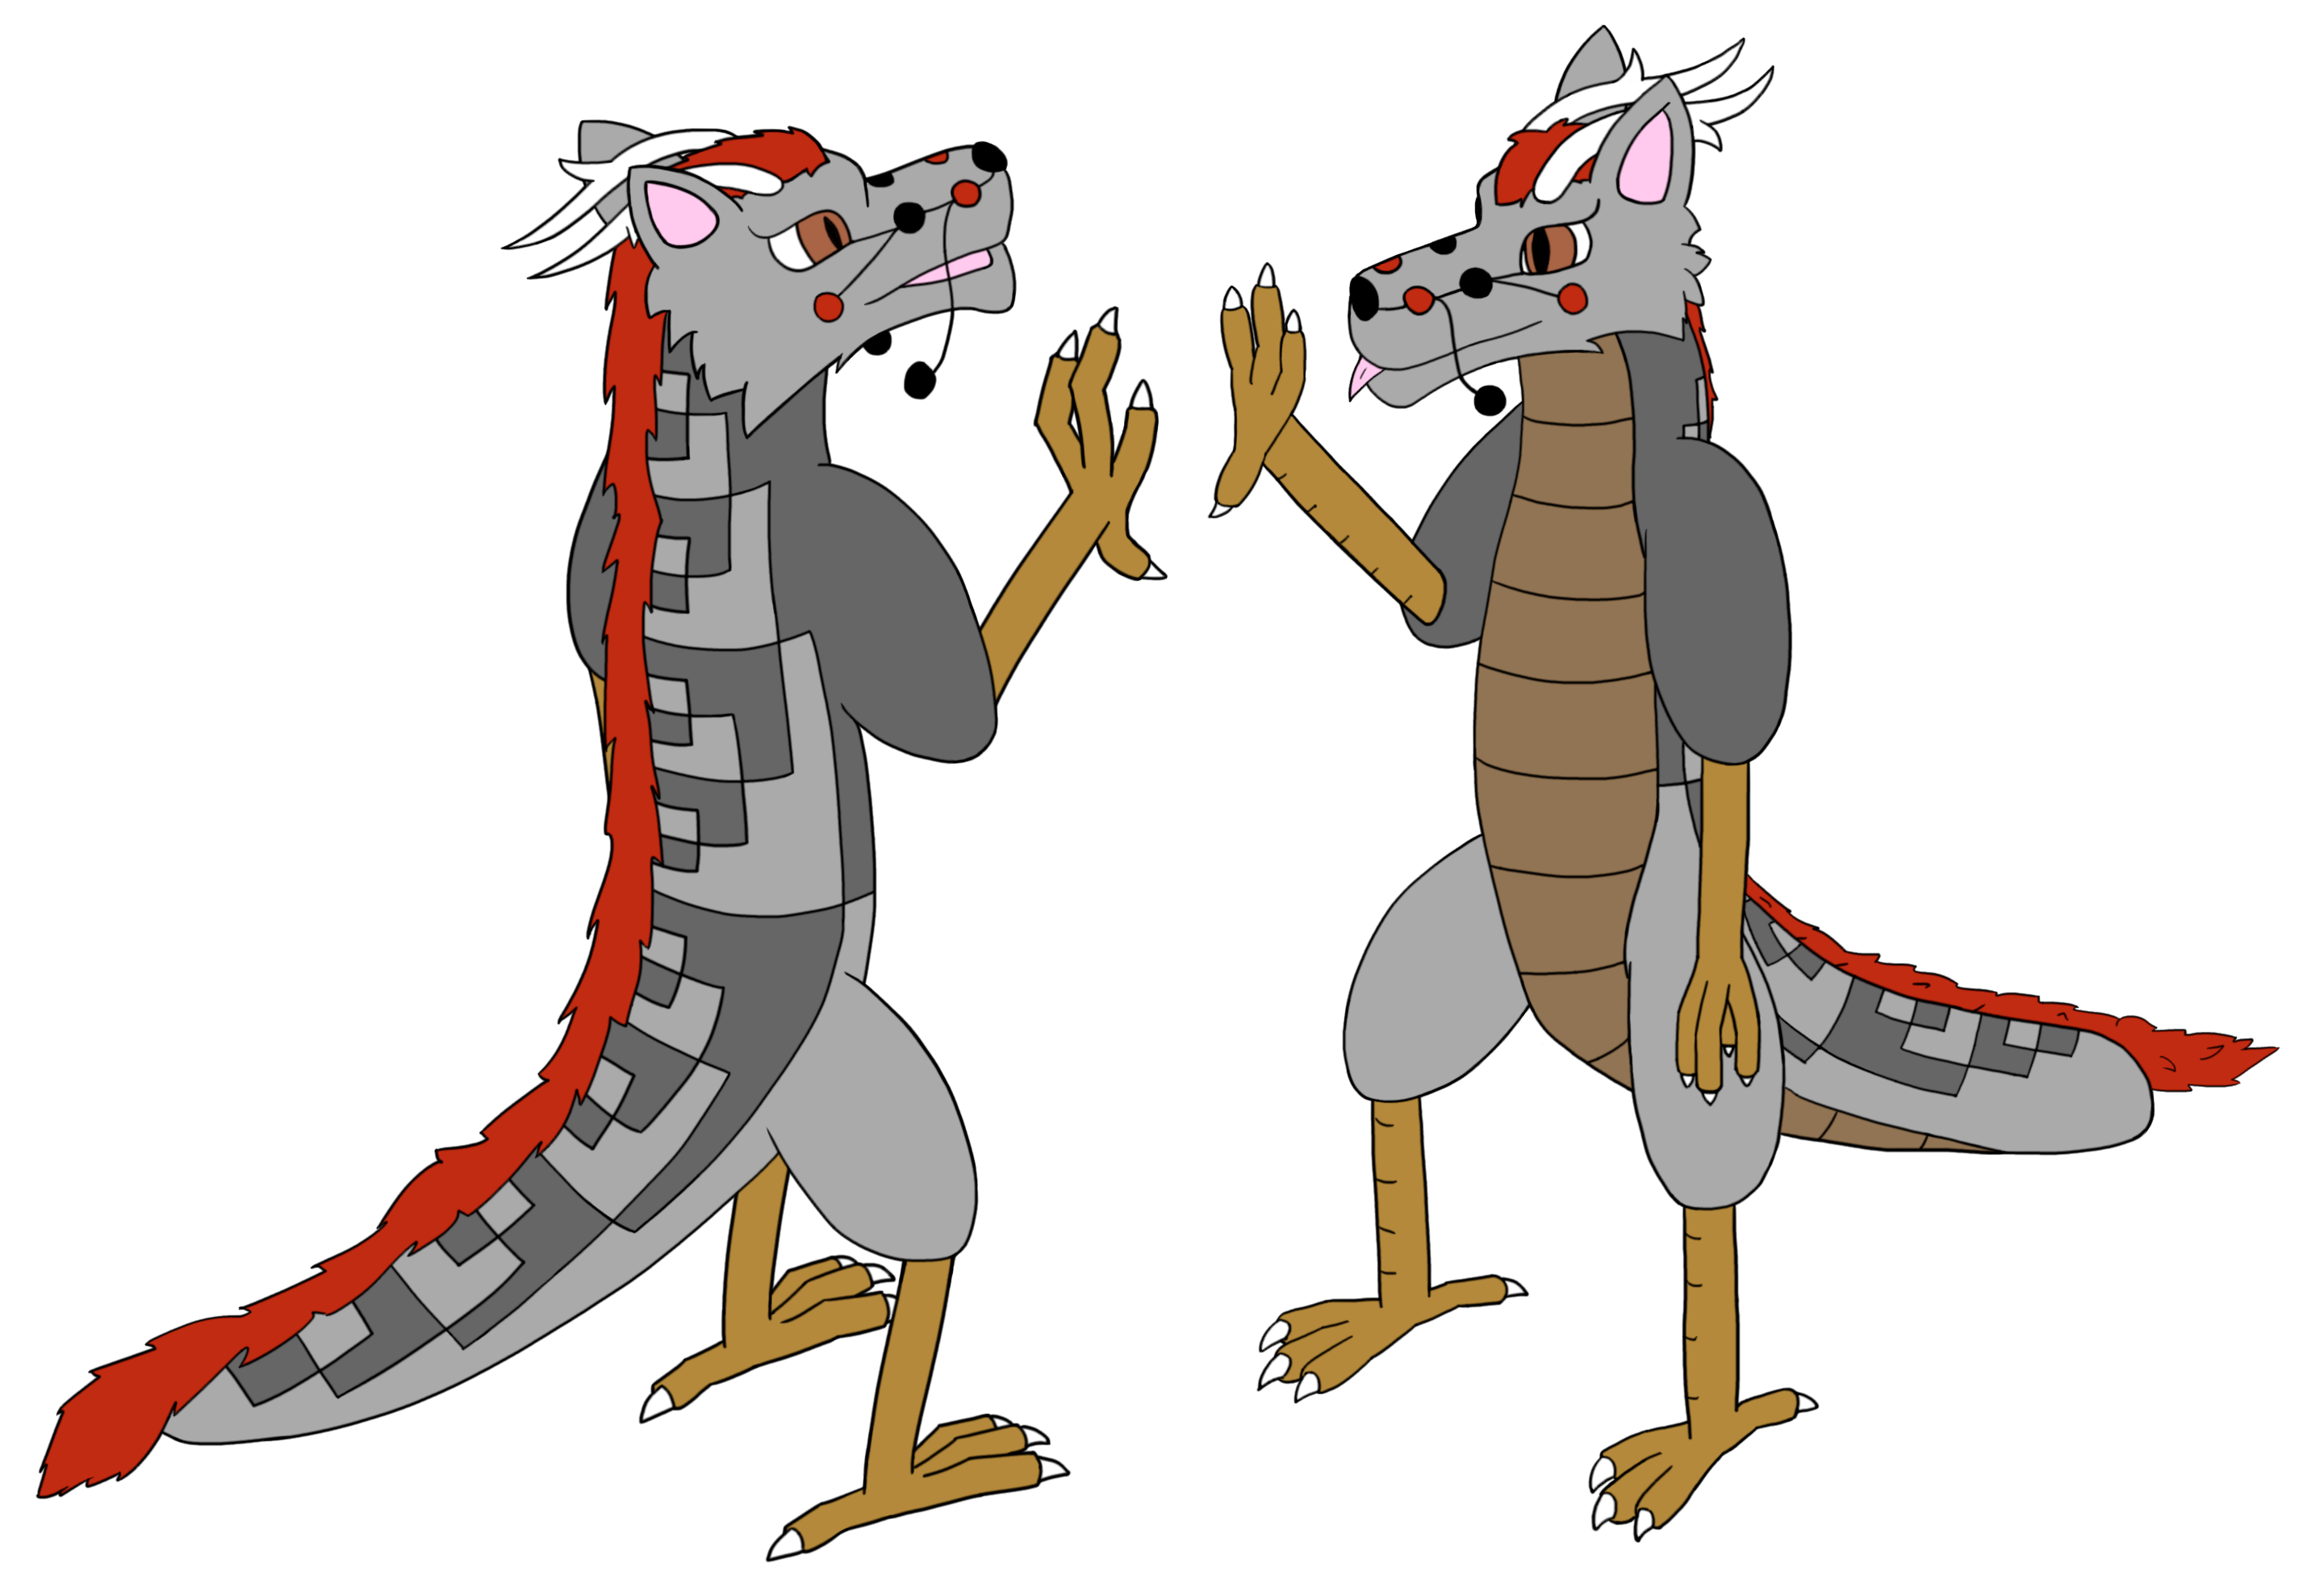
\includegraphics[width=\textwidth]{slides/unsigned_long/refsheet_bare.png}
\end{figure}

\end{overprint}

\end{columns}
}